\documentclass[12pt,a4paper,titlepage]{article}


\usepackage[MeX]{polski}       % polish suppot
\usepackage[utf8]{inputenc}    % utf8 support
\usepackage{graphicx}          % enable images input
\usepackage{wrapfig}           % enable wraping images
\usepackage{enumitem}          % control on enumerations
\usepackage{color}             % for color text

\usepackage[usenames,dvipsnames]{xcolor} % for more colors

% bottom paragraphs
\newenvironment{bottompar}{\par\vspace*{\fill}}{\clearpage}


% enable hyperlinks and set its properties
\usepackage[]{hyperref} % http://ctan.org/pkg/hyperref
\hypersetup{
    colorlinks,
    linkcolor={red!50!black},
    citecolor={blue!50!black},
    urlcolor={blue!80!black}
}

% separate captions for equations
\usepackage{caption}
\DeclareCaptionType{mycapequ}[Equation][List of equations]
\captionsetup[mycapequ]{labelformat=default}

% margins setup
\usepackage[top=2.5cm, bottom=2.5cm, left=3cm, right=3cm]{geometry}


% author and title
\title{\large{ARTIFICIAL NEURAL NETWORKS} \\
	\huge{\textsc{Multilayer Perceptron}}}
\author{Arkadiusz Gabryś \\
		Matrikel-Nr. 21895081 \\
		Department of Compuer Science}


% header and footer -------------------------------
\usepackage{fancyhdr}    % include package
\usepackage{lastpage}    % to get number of pages
\pagestyle{fancy}        % set style

% change header and footer width
\newlength\FHoffset
\setlength\FHoffset{0.6cm}

\addtolength\headwidth{2\FHoffset}
\fancyheadoffset{\FHoffset}
\fancyfootoffset{\FHoffset}

% header
\fancyhead{}                                   % clear header
\lhead{\textsc{Multilayer Perceptron}}         % write document title
\renewcommand{\sectionmark}[1]{\markright{#1}} % get rid of section number
\rhead{\rightmark}                             % print section name
\renewcommand{\headrulewidth}{0pt}             % get rid of the horizontal line

% footer
\fancyfoot{}                                   % clear footer
\fancyfoot[R]{\thepage~/~\pageref*{LastPage}}  % show page number on the right
\renewcommand{\footrulewidth}{0pt}             % get rid of the horizontal line
% -------------------------------------------------


\begin{document}

\maketitle                % create title

\thispagestyle{empty}     % remove page number from table of content
\begin{small}

\label{abstract}
\textbf{Abstract} --- content of this document describes simple and typical multilayer 

\end{small}

 % input Abstract without new line
\tableofcontents          % create table of content
\cleardoublepage          % flush all floats and create new page

\setcounter{page}{1}      % reset pages counter

\section{Introduction}
Many tasks involving mathematical models and equations cannot be solve by algorithm because of its complexity or limitations in computer calculations. Also such problems exist which are too difficult to be describe by math itself. Sometimes it is even not known if mathematical model exist.

Some of this tasks are trivial for humans and by simulating how the human brain works it is possible to create algorithm that is able to \textit{learn} how to solve a problem. \textit{Learning} mean that mathematical model modify itself in \textit{learning process} to meet certain conditions defined by \textit{training~set}. What is \textit{training set} and how \textit{learning process} is done will be covered in next chapters.

Now it is necessary to point that the way brain works is not fully known. But to create simple model our today knowledge is sufficient enough. Structure and mechanism of single neuron is know so based on that mathematical model can be create. Such model is just a generalization of something very complex. Yet good enough to reach our goals and break the bounders of what computer is capable of.

Algorithms uses neural network approach are relativity easy to understand and write in compare to what they can achieve. They are also quite fast. Because of that they are very popular in the filed of machines learning and problem solving.

Popularity of this method has led to creation of many variants and approaches in neural networks field. From ...
\section{Neuron}

\subsection{Cell}

\begin{figure}[!h]
    \centering
    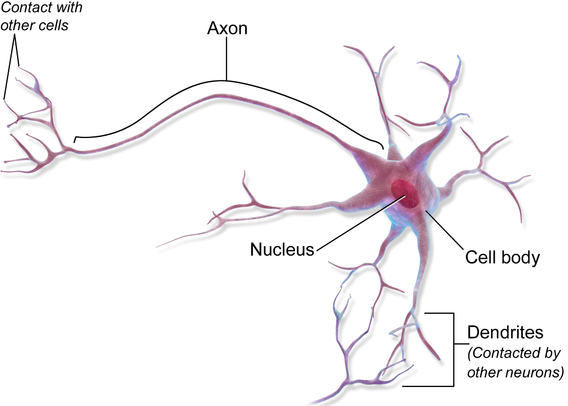
\includegraphics[scale=1]{Media/MultipolarNeuron.png}
    \caption[Multipolar neuron cell]{Multipolar neuron cell \textit{(sizes and shapes vary)}}
    \label{fig:MultipolarNeuronCell}
\end{figure}

Without going into a details. There exist a few type of neural cell. In our mathematical model we use \textit{Multipolar neural cell} which is shown on \hyperref[fig:MultipolarNeuronCell]{Figure \ref{fig:MultipolarNeuronCell}}. This one constitute the majority of neurons in the brain and include motor neurons and interneurons.

The way it works is such that it gather input signals through \textit{dendrites} and produce one output signal through \textit{axon}. The input signals are sum by \textit{nucleus} and only if specific value is obtains the \textit{axon} is activated. Both input and output signal are also modified while they are transmitted to \textit{nucleus} or next cell. Modification depends on \textit{nucleus} and thickness of \textit{neurolemma (which is not shown on the figure)}. This signal changing part is a place where the \textit{neurons network} knowledge is contained.

\newpage
\subsection{Model}

\begin{figure}[!h]
    \centering
    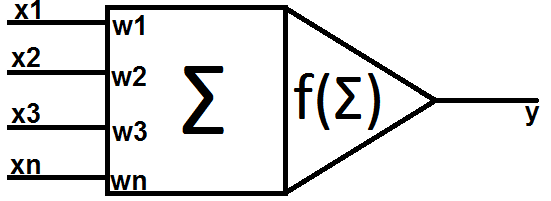
\includegraphics[scale=0.5]{Media/Neuron.png}
    \caption{Basic neuron/perceptron model}
    \label{fig:NeuronModel}
\end{figure}

Such \textit{multipolar neuron cell} mechanism can be easily model. Each \textit{neuron} input is represented by $x_n$ and multiply by corresponding factors $w_n$ (1) which represents change in \textit{neuron} input signal. All signals are sum (2) (that represents \textit{nucleus} function) and then processed by the \textit{activation function} (3) (which is representation of the active or inactive \textit{axon} and also serves other purposes - more about that later in this chapter).

\begin{eqnarray}
x_n \times w_n &=& \Delta_n \\
\sum\limits_{i=1}^n \Delta_i &=& \Sigma \\
f(\Sigma) &=& y
\end{eqnarray}

\begin{mycapequ}[!ht]
    $$f\left(\sum\limits_{i=1}^n x_iw_i\right) = y$$
    \caption{Basic neuron/perceptron model}
    \label{formula:NeuronMathModelEquation}
\end{mycapequ}

Most part of the model is simple and obvious yet the \textit{activation function} need to be discuss in more details.

\textit{Activation function} may take various form - from simple identity function to step function or more complicated continuous functions. It all depends on the output we want to obtain and/or the problem specification. In today's applications mostly sigmoidal continuous functions are used:

\begin{mycapequ}[!ht]
    $$y = sgm(x) = \frac{1}{1+e^{-\lambda s}}$$
    \caption{Sigmoidal activation function}
    \label{formula:SigmoidalActivationFunction}
\end{mycapequ}

Most of \textit{activation functions} are more or less similar. The $x$ is the sum calculated by neuron in step (2). On $\lambda$ depends slope of the function, in many cases this factor is omitted. 

\newpage

\begin{figure}[!h]
    \centering
    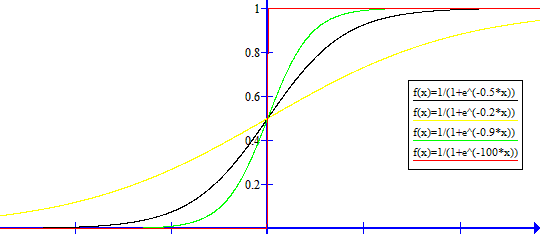
\includegraphics[scale=1]{Media/sgm_graph.png}
    \caption[Sigmoidal activation function graph]{Sigmoidal activation function graph with different lambda factors}
    \label{fig:SigmoidalFunctionGraph}
\end{figure}

Opis właściwości wzoru, które można zaobserwować na wykresie

\section{Network}

For one neuron there is one output value so we can easily see that one is not enough to solve many problems. Combining neurons into networks and layers will make them more useful. But one single neuron is still able to solve some class of problems.

\begin{wrapfigure}{r}{0.3\textwidth}
    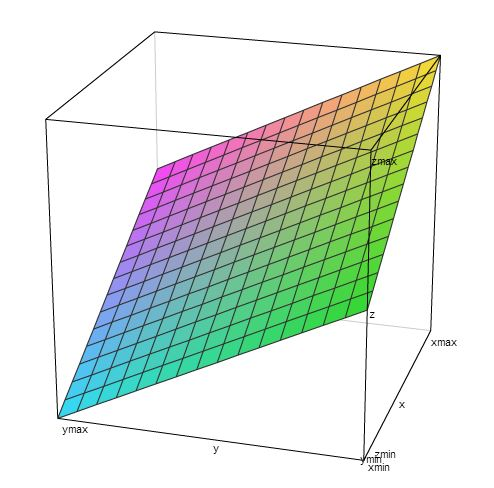
\includegraphics[width=0.32\textwidth]{Media/Plane.png}
    \caption{Single neuron plane}
    \label{fig:SingleNeuronPlane}
\end{wrapfigure}

Typically each neuron has one constant input value. Graphical interpretation of neuron can show why and also what class of problems can be solve with one neuron only.

Consider a neuron with three inputs $n = 3$ and with random weights $w_n$. So we have four axis, three for input data and one to show neuron output. Without one constant input graph of such neuron would be just a random set of points in 4D space.

But if we set one of the inputs constant then we will have only three axis, two for data and one for output value. Because of this one constant input instead of set of random points we will obtain 3D plane (\hyperref[fig:SingleNeuronPlane]{Figure \ref{fig:SingleNeuronPlane}}).

So our single neuron is able to model a $n$D planes. Such plane allows us to distinguish between three possibilities: data are greater then model, smaller or equal. It is enough to solve all linearly separable problems (e.g. logical AND, OR functions). But not all of the problems are linearly separable.


\subsection{Layers}

Before solving non linearly separable problems it have to be shown how more then one output can be obtain.

By putting same input values into multiple neurons with different set of weights $w_n$ a~more then one output can be obtain. Of course the single constant input still need to be provide for each of the neurons.

There are no differences between just using three separate neurons with different weights. So neurons in such configuration cannot solve problems beyond single neuron capabilities.

\begin{figure}[!h]
    \centering
    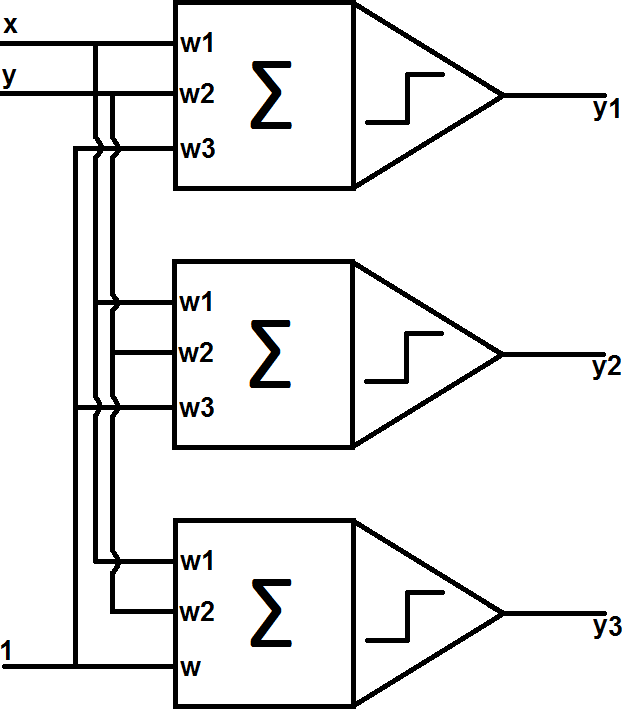
\includegraphics[scale=0.27]{Media/Layer.png}
    \caption[One layer of neurons]{One layer of neurons - two inputs with common constant one}
    \label{fig:OneNeuronsLayer}
\end{figure}

\newpage

\subsection{MLNN/PLP}

\begin{figure}[!h]
    \centering
    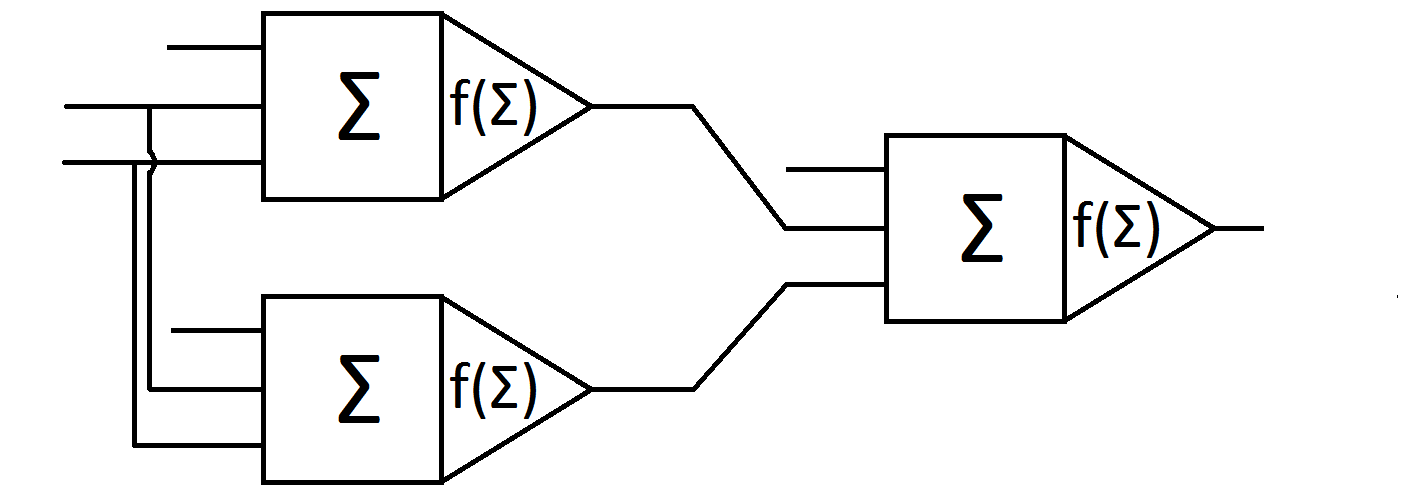
\includegraphics[scale=0.2]{Media/MLN.png}
    \caption[Multilayer network]{Very simple multilayer network}
    \label{fig:MLN}
\end{figure}

Non linearly separable problems can be solve by connecting multiple layers of neurons. \hyperref[fig:MLN]{Figure \ref{fig:MLN}} shows the simplest possible structure of \textit{Multilayer Perceptron}. Such structure is called \textit{Multilayer perceptron} or \textit{Feedforward neural network} or just \textit{Multilayer neural network}.

\textit{Feedforward neural network} is in our case the best naming convention because it tells exactly how each layer is connected. \textit{Feedforward} means that each output signal is connected only to next layer input. So no recursive connections, loops etc. Such network structure is most popular because we now how to train neurons in that structure. More about that in next \hyperref[sec:Training]{section}.

\begin{wrapfigure}[14]{r}{0.3\textwidth}
    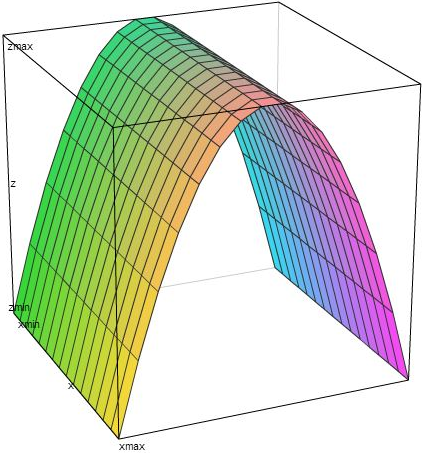
\includegraphics[width=0.32\textwidth]{Media/Bridge.png}
    \caption{Graph of three neurons combined in two layer structure}
    \label{fig:BridgeGraph}
\end{wrapfigure}

In general each multilayer network can be divided into three parts \cite{mlpPawelRosczak,mlpFSaC,fsmlpDwrSkrMk}:
\begin{itemize}
    \item \label{InputLayer} Input layer - used to prepare input data for network e.g. scaling or changing data distribution;
    \item \label{HiddenLayer} Hidden layers - actual \textit{feedforward network} with neurons; 
    \item \label{OutputLayer} Output layer - provides output data, can do some additional output preparation e.g. rescaling, swapping data;
\end{itemize}

\textit{Input layer} is in many cases omitted as well as \textit{output layer}.

The most important \textit{hidden layer} in \textit{feedforward network} has only one rule: \textit{connect output from $m$ layer to $m+1$ layer}. Not all of the output has to be connected to all neurons in next layer but this is usually the case. Still each of the neurons has to have its one constant input. Graph of such network (\hyperref[fig:BridgeGraph]{figure \ref{fig:BridgeGraph}}) will show why non linearly separable problems now can be model by such network.

\newpage
Now there is a question how many neurons and layers is needed. \\ There are two simple rules \cite{mlpPawelRosczak}:
\begin{enumerate}[topsep=8pt,itemsep=-1ex,partopsep=1ex,parsep=1ex]
    \item As small number of layers as possible
    \item As small number of neurons as possible
\end{enumerate}
And there are many approaches to solve this problem:
\begin{enumerate}[topsep=8pt,itemsep=-1ex,partopsep=1ex,parsep=1ex]
    \item Analytical calculations
    \item Building network from small number of neurons and measuring results
    \item Building network from large number of neurons and measuring results
    \item Generic algorithms
    \item Using theoretical knowledge about the problem
\end{enumerate}
None of this methods will be discussed here.

\begin{figure}[!h]
    \centering
    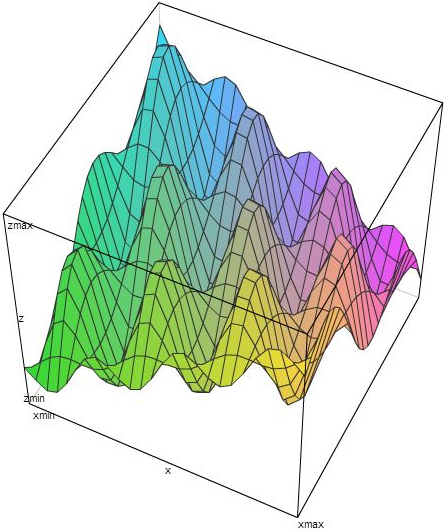
\includegraphics[scale=0.8]{Media/SolutionGraph.png}
    \caption{Complicated model modeled by MLP}
    \label{fig:SolutionGraph}
\end{figure}

\newpage
\subsection{Training}
\label{sec:Training}

Now the EBP\textit{(Error Back Propagation)} algorithm will be discussed \cite{mlpPawelRosczak,mlpFSaC,fsmlpDwrSkrMk,sRpNAI369}.
Training of multilayer network is numerical optimization of goal function $Q(k)$ where EBP algorithm in one of the gradient based methods.

\begin{mycapequ}[!ht]
    $$ {w_i}^{(n)}(k) = {w_i}^{(n)}(k-1)-\alpha\frac{\partial Q(k)}{{w_i}^{(n)}} $$
    \caption{Error Back Propagation \cite{mlpPawelRosczak}}
    \label{formula:EBP}
\end{mycapequ}

Using this formula we will for each iteration $k$ modify previous weight ${w_i}^{(n)}(k-1)$ of $i$ neuron in $n$ layer by negative gradient $\displaystyle{\alpha\frac{\partial Q(k)}{{w_i}^{(n)}}}$ where $\alpha$ is \textit{learn factor} (determine \textit{speed} of learning).
Goal function $Q(k)$ is usually square of the network result error.

\ 


To know network error the sample set with both inputs and results is needed. Such form of network training is called supervised. Creating good sample set is a~very large topic and wont be discussed here.

\section{Implementation}
\label{Implementation}

In this section will be presented simple $C\#$ program as an example implementation of presented topics.
By design it implements the simplest multilayer network with two inputs and one output to model boolean functions.
Program is capable to learn non linearly separable XOR function and show this process.

\subsection{User interface}
\label{UserInterface}

User interface presents the network structure.

\begin{figure}[!h]
    \centering
    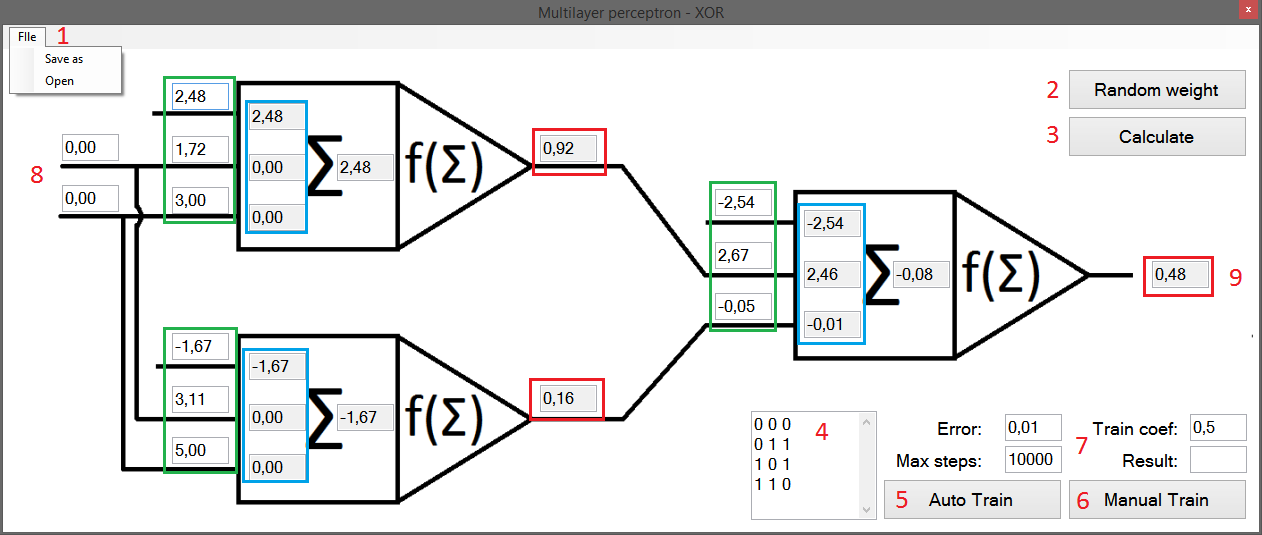
\includegraphics[scale=0.45]{Media/UI_numbers.png}
    \caption{User interface}
    \label{fig:UInumbers}
\end{figure}

Elements of interface:
\begin{enumerate}[topsep=8pt,itemsep=-1ex,partopsep=1ex,parsep=1ex]
    \item \label{FileMenu} File menu - save and open network configuration with training data
    \item \label{RandomWeight} Random weight - set random values for neurons weights
    \item Calculate - calculate network output for given input values (8)
    \item \label{TrainingData} Training data - first two values are network inputs third value is desired network output
    \item \label{AutoTrain} Auto train - train network using given Training data
    \item Manual train - perform one iteration of \hyperref[formula:EBP]{EBP algorith} with given input (8) and output given in Result field (7) as training data
    \item Training parameters:
    \begin{enumerate}[topsep=-1ex,itemsep=-1ex,partopsep=1ex,parsep=1ex]
        \item \label{Error} Error - desired error value for Auto training (5)
        \item \label{MaxSteps} Max steps - limits number of Auto training iterations
        \item \label{TrainCoef} Train coef - corresponds to \textit{learn factor} $\alpha$
        \item Result - desired network output value for Manual training
    \end{enumerate}
    \item Network inputs - used for Manual training (6) and for manual network output calculation (3)
    \item Network output - calculated when button Calculate is pressed (3)
\end{enumerate}

\textcolor{ForestGreen}{\textbf{Green}} elements are neurons weights, \textcolor{Cerulean}{\textbf{blue}} are multiplication of weights and inputs, \textcolor{red}{\textbf{red}} are neurons outputs.

\subsection{Program structure}
\label{ProgramStrucutre}

Whole project is accessible on \url{https://github.com/gabr/kisem_xor} \\
It is based on two classes \textit{XORForm} and \textit{Network}:

\begin{itemize}[topsep=1pt,itemsep=-1ex,partopsep=1ex,parsep=1ex]
    \item \textit{XORForm}:
    \begin{itemize}[topsep=0pt,itemsep=-1ex,partopsep=1ex,parsep=1ex]
        \item Implements \hyperref[UserInterface]{User interface} actions
        \item Contains \textit{Network} class 
    \end{itemize}
    \item \textit{Network}:
    \begin{itemize}[topsep=0pt,itemsep=-1ex,partopsep=1ex,parsep=1ex]
        \item Contains all neurons weights $w$, inputs $u$ and it sum of weighted inputs~$S$
        \item Properties \textit{Inputs} and \textit{Output} gives access to \hyperref[InputLayer]{first} and \hyperref[OutputLayer]{last} layer of network
        \item \textit{\_connections} is a list of tuples where one tuple represents one connection between neurons
        \item \textit{\_rand} is a object used to generate random values of weights
        \item Methods implements \hyperref[UserInterface]{User interface} actions and the \textit{Train()} method implements \hyperref[formula:EBP]{EBP algorith}
    \end{itemize}
\end{itemize}

Whole classes structure can be seen on \hyperref[fig:Classes]{Figure \ref{fig:Classes}}.

\begin{figure}[!h]
    \centering
    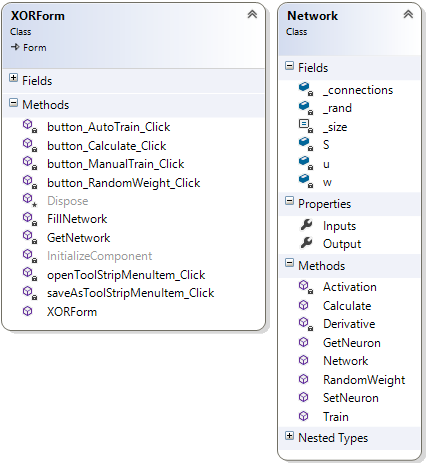
\includegraphics[scale=1]{Media/Class.png}
    \caption{Classes}
    \label{fig:Classes}
\end{figure}

\newpage

\subsection{Usage}
\label{Usage}

Usage of program on example of training boolean function XOR:
\begin{enumerate}[topsep=8pt,itemsep=-1ex,partopsep=1ex,parsep=1ex]
    \item \hyperref[UserInterface]{Open program}
    \item Set \hyperref[RandomWeight]{random weights}
    \item Provide true table for XOR function in \hyperref[TrainingData]{training data} window
    \item Set desired \hyperref[Error]{error} value and \hyperref[MaxSteps]{maximum iterations} value
    \item Set \hyperref[TrainCoef]{learning factor}
    \item Press \hyperref[AutoTrain]{Auto Train} button
\end{enumerate}

The resulted calculated weights can be saved using \hyperref[FileMenu]{File menu} \textit{File $\rightarrow$ Save as}.

\begin{figure}[!h]
    \centering
    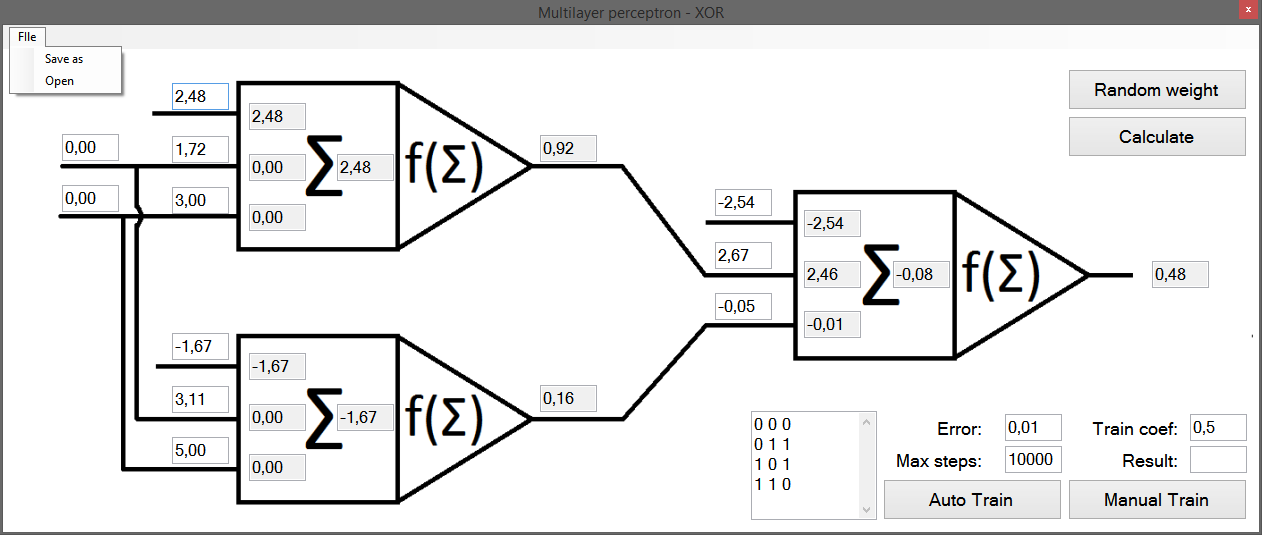
\includegraphics[scale=0.45]{Media/UI.png}
    \caption{Example results}
    \label{fig:ExampleUsage}
\end{figure}
\section{Observations and Conclusions}
\label{ObservationsConclusions}

As a summary some observations and conclusions related to topic will be presented.

\subsection{Limitations}
\label{Limitations}

Neural networks are perfect in creating mathematical models based on sample set and also without it (unsupervised learning) but they cannot model all functions. For example generation of random value cannot be achieve by neural network. Also choosing the proper sample set is a very difficult task itself and we need to be aware of \textit{overfitting} problem.

\hyperref[sec:Training]{Error Back Propagation} algorithm is very old and simple algorithm. It works but it is not perfect. It not guarantee reaching global minimum just a local one. Its also very sensitive to initial values of neuron weights. The criteria to stop algorithm are also not exactly clear. \\
There exist various modifications of pure \hyperref[sec:Training]{EBP} algorithm which solves some of this problems.

\subsection{Implementation}
\label{Implementation}

Neural network is described by mathematical tools so there is no strict way from equations to implementation.
But complexity of implementation is much lower in compare to theory and benefits of this neural networks algorithms are much larger than implementation effort.

Good advice for implementation is to \textbf{not} follow OOP standards and implement neurons as set of arrays and lists. This makes transition between mathematical description and code very easy, fast and produces less errors.


\subsection{Applications}
\label{Applications}

Ability to model very complex and unknown models makes neural networks perfect for all pattern recognition and decision making tasks such as: character recognition, image compression, stock market prediction. Recently was shown that large enough network with good sample set is able to perform face recognition task more accurate than humans.

It is also good tool for numerical approximation of complex and hard to calculate mathematical functions.
\addcontentsline{toc}{section}{References}
\begin{thebibliography}{9}
     
\bibitem{sRpNAI369}
    S. Russell, P. Norvig
    \emph{Artificial Intelligence, A modern Approach},
    3rd edition, PEARSON 2010 (pp.727-737)
    
\bibitem{mlpFSaC}
    Sankar K. Pal
    \emph{Multilayer Perceptron, Fuzzy Sets, and Classification}
    \emph{(09.1992)}
    
\bibitem{fsmlpDwrSkrMk}
    Dennis W. Ruck, Steven K. Rogers, Matthew Kabrisky
    \emph{Feature Selection Using a Multilayer Perceptron}
    \emph{(7.11.1989)}
    
\bibitem{manyNeuronVersions}
    Al, Martini, Frederic Et.
    \emph{Anatomy and Physiology}
    2007 Ed.2007 Edition. Rex Bookstore, Inc. p. 288  
    
\bibitem{mlpPawelRosczak}
     P. Rośczak
     \emph{Jednokierunkowe, wielowarstwowe sieci neuronowe i algorytm wstecznej propagacji błędu},
     source: \url{http://www.rosczak.com/mlp/mlp.html}
     \emph{(15.03.2015)}
    
\bibitem{facePR}
    Web: \emph{Facebook Creates Software That Matches Faces Almost as Well as You Do},
    source \url{http://www.technologyreview.com/news/525586/facebook-creates-software-that-matches-faces-almost-as-well-as-you-do/}
    \emph{(6.04.2015)}
  
\bibitem{neuronPNG}
    File: \emph{Blausen 0657 MultipolarNeuron.png},
    source \url{http://en.wikipedia.org/wiki/File:Blausen_0657_MultipolarNeuron.png}
    \emph{(15.03.2015)}

\end{thebibliography}

\end{document}

